\documentclass[../../main.tex]{subfiles}

\begin{document}
\problem{3}
\begin{wts}
Run \lstinline{nslookup} to obtain the IP address of \lstinline{www.wikipedia.org} by sending a query to \lstinline{8.8.4.4} which is the IP address of the google public DNS server.   
\end{wts}
\begin{proof}
3. Run nslookup to obtain the IP address of www.wikipedia.org by sending a query to 8.8.4.4 which is the IP address of the google public DNS server.
- 208.80.154.224\\
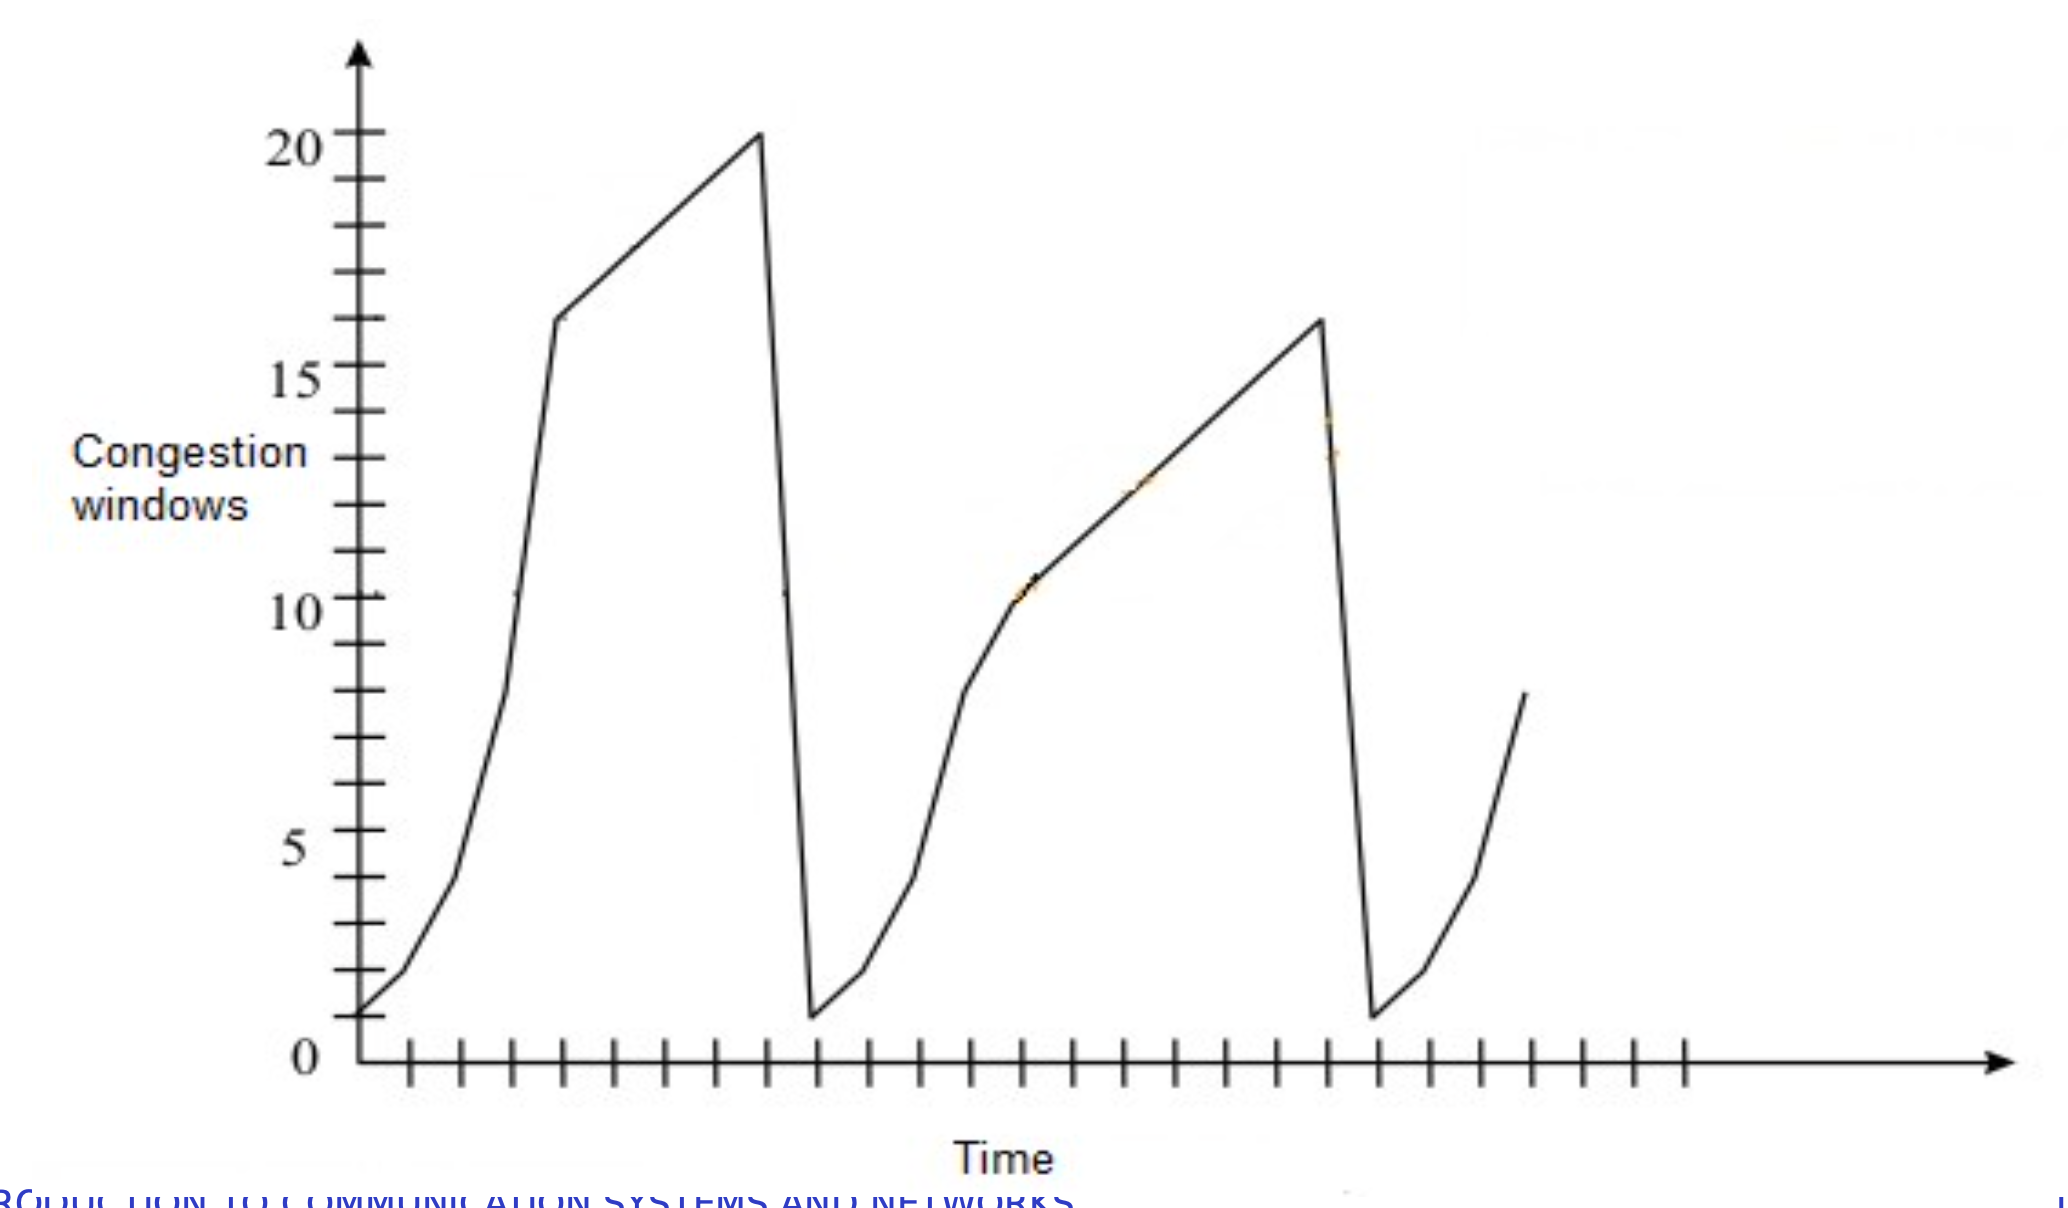
\includegraphics[width=\textwidth]{subfiles/images/part3_q19_window_graphic.png}
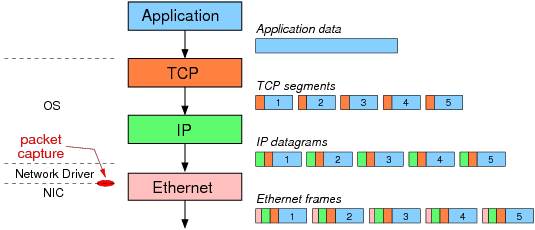
\includegraphics[width=\textwidth]{subfiles/images/L5_Manual/L5N2_ DNS & HTTP_PAGE24_13_Image153.png}
3. Run nslookup to obtain the IP address of www.wikipedia.org by sending a query to 8.8.4.4 which is the IP address of the google public DNS server.
- 208.80.154.224
\end{proof}

\end{document}